\section{Sucção} % (fold)
\label{sub:aspirador}
	
	Dentro dos principais objetivos, é necessário construir de forma objetiva um aspirador de pó. Deve-se projetar um sistema de sucção eficiente para que sugue desde de partículas de poeiras a resto de alimentos, estudo da dinâmica do processo, ou seja, o fluxo de ar dentro do motor do aspirador. Há dois tipos principais de modelos para ser utilizado em aspiradores de pó, um é o mais clássico utilizando ventiladores controlados por motores elétricos fazendo com que a pressão no interior do motor seja menor que a do ambiente e a diferença de pressão força o ar a entrar no aspirador seguindo até encontrar uma saída. Um filtro é colocado antes do ventilador para que seja separado a poeira do ar. O outro tipo é chamado de ciclone e não necessita de um filtro, pois pelo mesmo princípio da diferença de pressão o ar é sugado mas segue em uma trajetória helicoidal em torno de um cone e por efeito de força centrípeta a poeira é jogada para as paredes do aspirador e depois se depositam do inferior do aspirador onde são removidas, enquanto o ar percorre na direção contrária. \cite{layton}

	\subsection{Solução} % (fold)
	\label{sub:solução}
		
		Para o projeto foi escolhido o primeiro modelo do ventilador com filtro, pois  é uma solução com um custo menor e de fácil implementação se comparado ao sistema ciclone. Serão integradas nesse sistema escovas abaixo da linha de sucção, conhecidas como vassouras mágicas, que irão facilitar o transporte e direcionar a poeira para dentro do aspirador. Serão escolhidos dois coolers comerciais com uma vazão de ar por volta de 160 m\textsuperscript{3}/h, que serão colocados lado a lado dentro de um sistema hermeticamente fechado.

		A geometria do sistema busca diminuir a área de escoamento para aumentar a velocidade do fluído na ponta de sucção, utilizando do principio de conservação do fluxo de massa do sistema. O sistema de vedação será construído utilizando acrílico colado e mangueiras sanfonadas. Também será utilizado um motor para o acionamento da escova. Para o armazenamento do pó, será projetada uma caixa retangular de plástico com tampa. No momento da limpeza do depositório, o proprietário do aspirado deve apenas desencaixar a parte móvel, retirar as impurezas e encaixar novamente na tampa.

		O dispositivo de sucção da poeira está baseado na predição fornecida pela Equação da Continuidade. A equação descreve que o fluxo de massa que entra no sistema e o que sai no sistema é igual, de forma que a diminuição da seção transversal da tubulação causa um aumento da velocidade do escoamento, que por usa vez vai ter uma capacidade maior de arrastar partículas para dentro do sistema. Por sua vez, uma velocidade maior em um escoamento causa uma diminuição da pressão pelo princípio de Bernoulli e essa variação da pressão causa uma força que auxilia a aspiração de partículas.

		Os dados relativos ao fluxo de massa e potência dos coolers comerciais é muito limitado. Assim o dimensionamento do sistema será realizado utilizando uma simulação de base no Ansys em conjunto com experimentos empíricos em protótipos simplificados. Para primeira análise, foi realizada uma simulação com as condições de contorno definidas pelo fluxo de massa constante na entrada e na saída, com um valor de 0,026Kg/s ou  cerca de 50 CFM. A simulação mostrou uma velocidade de saída do escoamento de 5 m/s e a velocidade de entrada do ar de 19 m/s.

		\begin{figure}[H]
			\centering
			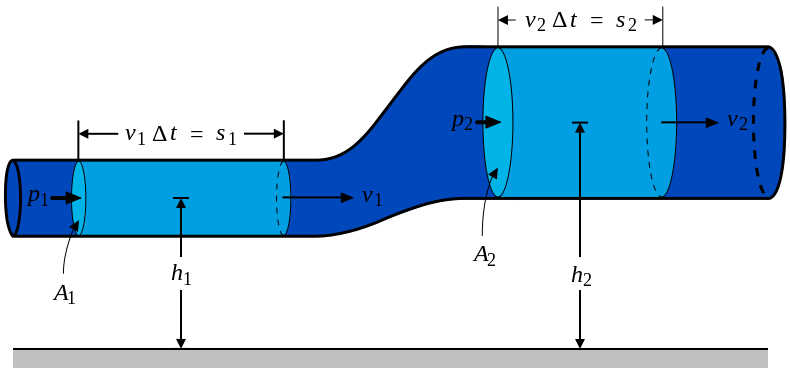
\includegraphics[scale=0.4]{figuras/succao.png}
			\caption{Demonstração da equação da continuidade, equação que descreve a conservação de massa do escoamento.}
			\label{img:succao}
		\end{figure}

		\begin{equation}\label{1}
		\frac{v^{2}}{2} + gh + \frac{p}{\rho} = constante
		\end{equation}
		
		ou
		
		\begin{equation}
		\frac{\rho v^{2}}{2} + \rho gh + p = constante
		\end{equation}

		$v$ = velocidade do fluido ao longo do condutor

		$g$ = aceleração da gravidade
		
		$h$ = altura em relação a um referencial
		
		$p$ = pressão ao longo do recipiente
		
		$\rho$ = massa específica do fluido

		Segue a equação da continuidade na sua forma de integral:

		\begin{equation}
		\frac{dq}{dt} + \iint_{s}^{ }j . dS= \sum
		\end{equation}
		
		onde $S$ é qualquer superficie fechada imaginária, com um volume V;

		$\iint_{s}^{ }dS$ se refere a integral de superficie sobre a superficie fechada

		$q$ é o amontoado total do volume

		$j$ é o fluxo de q

		$t$ é o tempo


		A analise do fluxo de massa realizada no software \textit{Ansys} está apresentada na Figura \ref{img:analise_fluxo}.

		\begin{figure}[H]
			\centering
			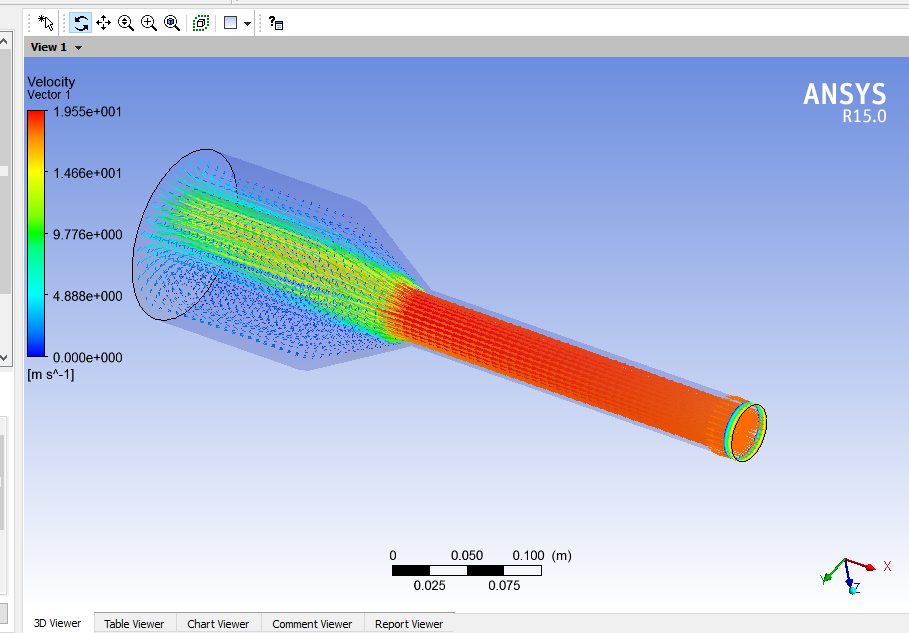
\includegraphics[scale=0.4]{figuras/analise_fluxo.png}
			\caption{Simulação do Ansys com o fluxo de massa de um cooler comercial.}
			\label{img:analise_fluxo}
		\end{figure}



	% subsection solução (end)
% section aspirador (end)